% Model 1 structure (paper Fig. "Structure of Model 1").
% Same content as Reports/M1/m1_structure.tex, recoloured by physical role with
% the shared paper palette: water = teal, vegetation = green, wind/sand = brown.
% Build: cd Paper/Figure && pdflatex m1_structure.tex
\documentclass[tikz,border=3pt]{standalone}
\usepackage{newtxtext,newtxmath}
\usepackage{amsmath}
\usetikzlibrary{arrows.meta,calc,backgrounds}
% Shared colours for the TikZ schematics; same roles and hex values as
% Code/figures_matlab/paper_style.m (mycolor.space, base #1E5F74).
%   water (P, I, M, W-bar)  teal   | vegetation (V, r, d)  green
%   wind and sand (E, S)    brown  | highlight             orange
%   limits and caps         red dashed
\definecolor{pWater}{HTML}{1E5F74}
\definecolor{pWaterMid}{HTML}{659FB6}
\definecolor{pWaterLight}{HTML}{DCEBF1}
\definecolor{pTeal}{HTML}{00828C}
\definecolor{pVeg}{HTML}{2B633C}
\definecolor{pVegMid}{HTML}{4AC087}
\definecolor{pVegLight}{HTML}{E3F3E8}
\definecolor{pSand}{HTML}{8F7159}
\definecolor{pSandLight}{HTML}{FFEACE}
\definecolor{pAccent}{HTML}{F49431}
\definecolor{pPV}{HTML}{D47216}
\definecolor{pPVLight}{HTML}{FDF1E3}
\definecolor{pPlum}{HTML}{7A437F}
\definecolor{pPlumLight}{HTML}{F2EBF3}
\definecolor{pLimit}{HTML}{D03B3B}
\definecolor{pInk}{HTML}{1F2B33}
\definecolor{pAxis}{HTML}{344A53}
\definecolor{pGrey}{HTML}{97AFB9}
\definecolor{pGreyDark}{HTML}{647B84}
\definecolor{pGrid}{HTML}{E6EBED}

\tikzset{
  box/.style={rectangle, rounded corners=2.5pt, line width=0.8pt, align=center,
    font=\small, inner xsep=4pt, inner ysep=3pt, minimum height=0.78cm,
    execute at begin node={\hyphenpenalty10000 }},
  % data: white chip with a coloured edge
  data/.style={box, draw=#1, fill=white, text=pInk},
  % derived quantity or method: light tint, coloured edge
  step/.style={box, draw=#1, fill=#1!10, text=pInk},
  % model core: solid colour, white bold text
  core/.style={box, draw=#1, fill=#1, text=white, font=\small\bfseries, minimum height=0.95cm},
  % result: dark colour, white text
  result/.style={box, draw=#1, fill=#1, text=white},
  flow/.style={-{Stealth[length=5pt,width=4pt]}, line width=0.8pt, draw=#1},
  flow/.default=pAxis,
  colhead/.style={font=\footnotesize\bfseries, text=pGreyDark, anchor=south},
}
\begin{document}
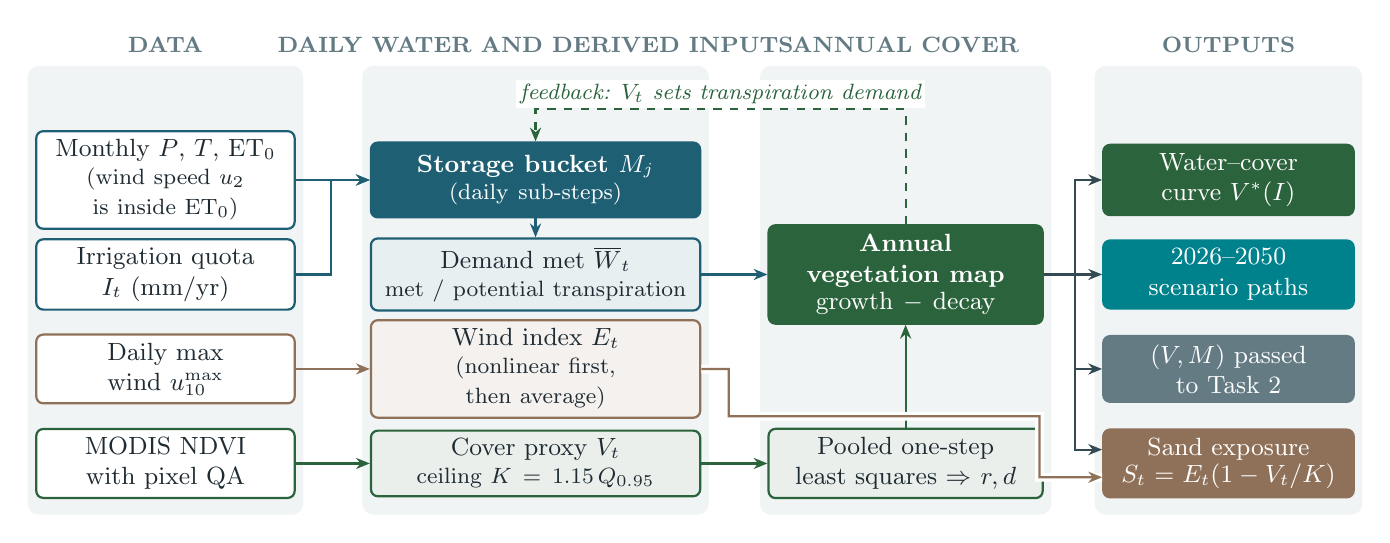
\begin{tikzpicture}
% ---- column headings
\node[colhead] at (1.85,0.55)  {DATA};
\node[colhead] at (6.55,0.55)  {DAILY WATER AND DERIVED INPUTS};
\node[colhead] at (11.25,0.55) {ANNUAL COVER};
\node[colhead] at (15.35,0.55) {OUTPUTS};

% ---- inputs (column 1)
\node[data=pWater, text width=3.0cm] (clim) at (1.85,-0.95) {Monthly $P$, $T$, ET$_0$\\[-1pt]{\footnotesize (wind speed $u_2$ is inside ET$_0$)}};
\node[data=pWater, text width=3.0cm] (irr)  at (1.85,-2.15) {Irrigation quota $I_t$ (mm/yr)};
\node[data=pSand,  text width=3.0cm] (wind) at (1.85,-3.35) {Daily max wind $u_{10}^{\max}$};
\node[data=pVeg,   text width=3.0cm] (ndvi) at (1.85,-4.55) {MODIS NDVI with pixel QA};

% ---- derived quantities and water module (column 2)
\node[core=pWater, text width=3.9cm] (bucket) at (6.55,-0.95) {Storage bucket $M_j$\\[-1pt]{\footnotesize\normalfont (daily sub-steps)}};
\node[step=pWater, text width=3.9cm] (wbar) at (6.55,-2.15) {Demand met $\overline W_t$\\[-1pt]{\footnotesize met / potential transpiration}};
\node[step=pSand,  text width=3.9cm] (eidx) at (6.55,-3.35) {Wind index $E_t$\\[-1pt]{\footnotesize (nonlinear first, then average)}};
\node[step=pVeg,   text width=3.9cm] (cover) at (6.55,-4.55) {Cover proxy $V_t$\\[-1pt]{\footnotesize ceiling $K=1.15\,Q_{0.95}$}};

% ---- vegetation map and calibration (column 3)
\node[core=pVeg, text width=3.2cm, minimum height=1.25cm] (veg) at (11.25,-2.15) {Annual vegetation map\\[-1pt]{\normalfont growth $-$ decay}};
\node[step=pVeg, text width=3.2cm] (cal) at (11.25,-4.55) {Pooled one-step least squares $\Rightarrow r,d$};

% ---- outputs (column 4)
\node[result=pVeg,   text width=2.9cm] (curve) at (15.35,-0.95) {Water--cover curve $V^*(I)$};
\node[result=pTeal,  text width=2.9cm] (scen)  at (15.35,-2.15) {2026--2050 scenario paths};
\node[result=pGreyDark, text width=2.9cm] (iface) at (15.35,-3.35) {$(V,M)$ passed to Task 2};
\node[result=pSand,  text width=2.9cm] (sand)  at (15.35,-4.55) {Sand exposure\\[-1pt]$S_t=E_t(1-V_t/K)$};

% ---- flows
\draw[flow=pWater] (clim.east) -- (bucket.west);
\draw[flow=pWater] (irr.east) -- ++(0.45,0) |- (bucket.west);
\draw[flow=pSand] (wind.east) -- (eidx.west|-wind.east);
\draw[flow=pVeg] (ndvi.east) -- (cover.west|-ndvi.east);
\draw[flow=pWater] (bucket) -- (wbar);
\draw[flow=pWater] (wbar.east) -- (veg.west|-wbar.east);
\draw[flow=pVeg] (cover.east) -- (cal.west);
\draw[flow=pVeg] (cal) -- (veg);
% wind index goes to the sand output only, never into the vegetation map;
% the white casing lets it hop over the calibration arrow
\draw[flow=pSand, preaction={draw=white, line width=3.2pt, -}] (eidx.east) -- ++(0.35,0) -- ++(0,-0.6) -- (12.95,-3.95) |- ([yshift=-5pt]sand.west);
\draw[flow=pVeg, dashed] (veg.north) -- (11.25,-0.05) -- node[above, font=\footnotesize\itshape, text=pVeg, fill=white, inner sep=1.5pt] {feedback: $V_t$ sets transpiration demand} (6.55,-0.05) -- (bucket.north);
\draw[flow] (veg.east) -- (scen.west);
\draw[flow] (veg.east) -- ++(0.4,0) |- (curve.west);
\draw[flow] (veg.east) -- ++(0.4,0) |- (iface.west);
\draw[flow] (veg.east) -- ++(0.4,0) |- ([yshift=5pt]sand.west);

% ---- light column bands behind the boxes
\begin{scope}[on background layer]
  \foreach \x/\w in {1.85/3.5, 6.55/4.4, 11.25/3.7, 15.35/3.4}
    \fill[pGrid!55, rounded corners=4pt] (\x-\w/2,0.5) rectangle (\x+\w/2,-5.2);
\end{scope}
\end{tikzpicture}
\end{document}
